\documentclass[a4paper,12pt, oneside]{book}

% \usepackage{fullpage}
\usepackage[italian]{babel}
\usepackage[utf8]{inputenc}
\usepackage{amssymb}
\usepackage{amsthm}
\usepackage{graphics}
\usepackage{amsfonts}
\usepackage{listings}
\usepackage{amsmath}
\usepackage{amstext}
\usepackage{engrec}
\usepackage{rotating}
\usepackage{verbatim}
\usepackage[safe,extra]{tipa}
\usepackage{showkeys}
\usepackage{multirow}
\usepackage{hyperref}
\usepackage{microtype}
\usepackage{fontspec}
\usepackage{enumerate}
\usepackage{braket}
\usepackage{marginnote}
\usepackage{pgfplots}
\usepackage{cancel}
\usepackage{polynom}
\usepackage{booktabs}
\usepackage{enumitem}
\usepackage{framed}
\usepackage{pdfpages}
\usepackage{pgfplots}
\usepackage{algorithm}
% \usepackage{algpseudocode}
\usepackage[cache=false]{minted}
\usepackage{mathtools}
\usepackage[noend]{algpseudocode}
\usepackage{tikz}\usetikzlibrary{er}\tikzset{multi  attribute /.style={attribute
    ,double  distance =1.5pt}}\tikzset{derived  attribute /.style={attribute
    ,dashed}}\tikzset{total /.style={double  distance =1.5pt}}\tikzset{every
  entity /.style={draw=orange , fill=orange!20}}\tikzset{every  attribute
  /.style={draw=MediumPurple1, fill=MediumPurple1!20}}\tikzset{every
  relationship /.style={draw=Chartreuse2,
    fill=Chartreuse2!20}}\newcommand{\key}[1]{\underline{#1}} 


\usepackage{fancyhdr}
\pagestyle{fancy}
\fancyhead[LE,RO]{\slshape \rightmark}
\fancyhead[LO,RE]{\slshape \leftmark}
\fancyfoot[C]{\thepage}


\title{Metodi Formali}
\author{UniShare\\\\Davide Cozzi\\\href{https://t.me/dlcgold}{@dlcgold}}
\date{}

\pgfplotsset{compat=1.13}
\begin{document}
\maketitle

\definecolor{shadecolor}{gray}{0.80}
\setlist{leftmargin = 2cm}
\newtheorem{teorema}{Teorema}
\newtheorem{definizione}{Definizione}
\newtheorem{esempio}{Esempio}
\newtheorem{corollario}{Corollario}
\newtheorem{lemma}{Lemma}
\newtheorem{osservazione}{Osservazione}
\newtheorem{nota}{Nota}
\newtheorem{esercizio}{Esercizio}
\algdef{SE}[DOWHILE]{Do}{doWhile}{\algorithmicdo}[1]{\algorithmicwhile\ #1}
\tableofcontents
\renewcommand{\chaptermark}[1]{%
  \markboth{\chaptername
    \ \thechapter.\ #1}{}}
\renewcommand{\sectionmark}[1]{\markright{\thesection.\ #1}}
\newcommand{\floor}[1]{\lfloor #1 \rfloor}

\chapter{Introduzione}
\textbf{Questi appunti sono presi a lezione. Per quanto sia stata fatta
  una revisione è altamente probabile (praticamente certo) che possano
  contenere errori, sia di stampa che di vero e proprio contenuto. Per
  eventuali proposte di correzione effettuare una pull request. Link: }
\url{https://github.com/dlcgold/Appunti}.\\
\textbf{Grazie mille e buono studio!}
\section{Contenuti del Corso}
\textit{Il corso tratta di metodi e tecniche formali per specificare, disegnare e
  analizzare sistemi complessi, in particolare sistemi concorrenti e distribuiti
  costituiti da componenti che operano in modo indipendente e che interagiscono
  tra loro.} \\ \\
Si usa un linguaggio logico che spiega il comportamento di tali sistemi e fa
riferimento alla \textbf{logica temporale} di tali sistemi, in quanto le
proprietà di tali sistemi sono tali per cui evolvono con il cambiamento di stato
del sistema e quindi serve una logica che descriva le proprietà dell'evoluzione
del comportamento.\\
Si parlerà delle \textbf{Reti di Petri}, ovvero uno strumento per modellare tali
sistemi concorrenti e distribuiti. Questo modello ha intrinsechi dei teoremi
matematici atti a studiare il comportamento di tali sistemi.\\
In laboratorio si studieranno algoritmi e strumenti software per la modellazione
e l'analisi di tali sistemi.\\
Si introducono a che sistemi dinamici a tempi discreti, come gli \textbf{automi
  cellulari}.
\chapter{Sviluppo di Modelli e Sistemi}
Si hanno diverse fasi di sviluppo di \textit{sistemi complessi} (nel nostro caso
\textbf{concorrenti} e \textbf{distribuiti}). Si hanno 4 grandi fasi (che
riprendono le generiche fasi dello sviluppo software), che non
seguono una rigida sequenza cronologica tra di loro:
\begin{enumerate}
  \item specifica del problema e delle proprietà della soluzione
  \item modellazione della soluzione
  \item implementazione
  \item verifica, validazione e collaudo, sia sul modello che
  implementazione (con eventuali modifiche)
\end{enumerate}
\textbf{Queste fasi possono alternarsi a vicenda}.\\
\textit{I metodi formali possono svolgere una parte rilevante in tutte queste 4
  fasi e hanno la prerogativa di sviluppare questi sistemi in maniera corretta e
  persistente.} \\
Ci si focalizza sulla modellazione e sulla specifica delle proprietà. Si studia
inoltre la verifica delle proprietà sul modello costruito. \textit{In questo
  corso si lascia un attimo da parte l'aspetto implementativo, che comunque
  seguirebbe alla verifica e alla validazione del metodo}.\\
% note sull'utilità dei metodi formali su elearning e sul loro uso
Si hanno diversi modelli di sistemi concorrenti e distribuiti, presenti in
letteratura: 
\begin{itemize}
  \item \textbf{Algebre di Processi}, ovvero una miriade di diversi linguaggi,
  studiate inizialmente da Milner, che introdusse il calcolo dei sistemi
  comunicanti, un calcolo algebrico utile alla semantica della
  concorrenza. Inoltre Hoare ha introdotto i \textbf{processi sequenziali
    comunicanti} come un nucleo di linguaggio di programmazione, usato come
  linguaggio macchina per le prime macchine parallele. Queste algebre si basano
  sul paradigma di avere un forte aspetto della \textbf{composizionalità}, in
  quanto un sistema viene visto come costituito da diverse componenti autonome
  (sia hardware, che software, che umane) che interagiscono tra loro
  sincronizzandosi (in modo sincrono, \textit{handshaking}, sfruttando un ``canale di comunicazione''
  che viene modellato come un processo) e scambiandosi messaggi. Questo
  paradigma è anche alla base dello sviluppo di molti linguaggi di
  programmazione specificatamente dedicati alla concorrenza.
  \item \textbf{Automi a Stati Finiti}. Un modello concorrente e distribuito
  viene spesso rappresentato attraverso \textbf{sistemi di transizioni
    etichettati}, che sono una derivazione del modello degli automi a stati
  finiti, già usati in letteratura per modellare reti neurali, progettare
  circuiti asincroni, modellare macchine a stati finiti, riconoscere linguaggi
  regolari (il teorema di Kleene ci ricorda che \textit{ad un automa a stati
    finiti è possibile associare un'espressione regolare}) e per la modellazione
  di protocolli di comunicazione. 
  \item \textbf{Reti di Petri}, introdotte da Petri con la \textbf{teoria
    generale delle reti di Petri} nella sua tesi di dottorato. Questa teoria
  parte da una critica al modello a stati finiti dove il focus è su stati
  globali e trasformazione di stati globali. Petri cercava invece una teoria
  matematica (fondata sui principi della fisica moderna della relatività e della
  quantistica) che fosse una teoria dei sistemi in grado di descrivere sistemi
  complessi in cui mettere al centro il flusso di informazione e che potesse
  permettere di analizzare l'organizzazione dal punto di vista del flusso di
  informazione che passa da una componente all'altra. Non si ha il focus,
  quindi, su ``macchine calcolatrici'' ma come supporto alla comunicazione in
  organizzazioni complesse. Si hanno quindi diversi elementi chiave:
  \begin{itemize}
    \item la comunicazione
    \item la sincronizzazione tra componenti
    \item il flusso di informazione che passa tra le varie componenti
    \item la relazione di concorrenza e l'indipendenza causale tra i vari eventi
    che comportano i cambiamenti di stato. Ci si concentra su stati locali
    e non sulla visione di una sequenza di azioni e di uno stato globale
  \end{itemize}
  La teoria delle reti di Petri è stata poi sviluppata e ha avuto diverse
  applicazioni. Sono stati sviluppati diversi linguaggi, ovvero diverse
  \textbf{classi di reti di Petri} per descrivere un sistema complesso a livelli
  differenti di astrazione. \\
  Sono state anche sviluppate tecniche formali di analisi e di verifica del
  modello (disegnato mediante reti di Petri), basate sulla teoria dei grafi e
  sull'algebra lineare.\\
  Le reti di Petri hanno avuto un notevole utilizzo in diversi ambiti
  applicativi anche estranei all'informatica pura e allo studio della
  concorrenze, come la modellazione di sistemi biologici o la modellazione di
  reazioni chimiche. Mediante una classe di reti particolare, le \textbf{reti
    stocastiche} si può valutare le prestazioni di un determinato modello.
\end{itemize}
\subsubsection{Sistemi di Transizioni Etichettati}
\begin{definizione}
  I sistemi di transizione etichettati sono definiti come gli automi a stati
  finiti ma senza essere visti come riconoscitori di linguaggi infatti un sistema
  è formato da un insieme, solitamente finito, di stati globali $S$. Si ha poi un
  \textit{alfabeto} delle possibili azioni che può eseguire il sistema. Si hanno
  anche delle relazioni di transizioni, ovvero delle transizioni che permettono di
  specificare come, attraverso un'azione, si passa da uno stato ad un altro. Le
  transizioni si rappresentano con archi etichettati tra i nodi, che rappresentano
  gli stati. Le etichette degli archi rappresentano le azioni necessarie alla
  trasformazione. L'insieme delle azioni viene chiamato $E$ mentre $T\subseteq
  S\times E\times S$ è l'insieme degli archi etichettati. Può essere,
  opzionalmente, individuato uno stato iniziale $s_0$. Un sistema non è obbligato
  a ``terminare'', quindi non si ha obbligatoriamente uno stato finale.\\
  Riassumendo quindi un sistema di transizione etichettato è un quadrupla:
  \[A=(S,E,T,s_0)\]
  \begin{figure}[H]
    \centering
    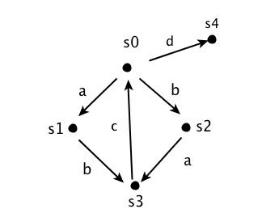
\includegraphics[scale = 0.5]{img/ste.jpg}
    \caption{Esempio di sistema di transizione etichettato}
  \end{figure}
\end{definizione}
La critica di Petri è che in un sistema distribuito non sia individuabile uno
\textbf{stato globale}, che in un sistema distribuito le trasformazioni di stato
siano \textbf{localizzate} e non globali, che non esista un sistema di
riferimento temporale unico (si possono avere più assi temporali in un sistema
distribuito). Quindi la simulazione sequenziale non deterministica (emantica a
``interleaving'') dei sistemi distribuiti è una forzatura e non rappresenta le
reali caratteristiche del comportamento del sistema, ovvero la località, la
distribuzione degli eventi e la relazione di dipendenza causale e non causale
tra gli eventi.
\section{Sistemi Elementari}
Per introdurre i sistemi elementari delle reti di Petri, ovvero una classe molto
semplice e astratta partiamo da un esempio:
\begin{esempio}
  Vediamo l'esempio del \textit{Produttore e del Consumatore}.\\
  Si ha un sistema con una componente Produttore che produce elementi e li
  deposita in un buffer che ha un'unica posizione (quindi o è pieno o è vuoto) e
  con un consumatore che preleva dal buffer un elemento per poi consumarlo ed
  essere pronto a prelevare un altro elemento. Si ha un comportamento
  ciclico. Usiamo quindi le reti di Petri, col modello dei sistemi elementari,
  per rappresentare questo modello. Bisogna quindi individuare le proprietà
  fondamentali locali del sistema.\\
  Partiamo dal produttore, che può avere 2 stati locali:
  \begin{enumerate}
    \item pronto per produrre
    \item pronto per depositare
  \end{enumerate}
  Usiamo i \textbf{cerchi} per rappresentare condizioni locali che sono
  associabili a delle proposizioni della logica che possono essere vere o
  false. Queste preposizioni sono quindi stati locali. Gli eventi locali vengono
  invece rappresentati con un \textbf{rettangolo}. Un evento ha un arco entrante
  da uno stato che rappresenta le \textit{precondizioni} di quell'evento (che
  devono essere vere per permettere l'occorrenza dell'evento). L'occorrenza
  dell'evento rende false le precondizioni e rende vere le
  \textit{postcondizioni} (che sono stati raggiungibili con un arco uscente da
  un evento). Si ha quindi che il produttore può depositare solo se il buffer
  non è pieno, quindi le postcondizioni di un evento devono essere false
  affinché l'evento possa occorrere (oltre alle precondizioni vere).\\
  Passiamo al consumatore che estrae solo se il buffer è pieno ed è pronto a
  prelevare. Si procede poi con la stessa logica del produttore di cambiamento
  tra vero e falso delle varie condizioni locali.\\
  In questo esempio si hanno quindi condizioni che sono preposizioni booleane e
  rappresentano stati locali.
  \begin{figure}[H]
    \centering
    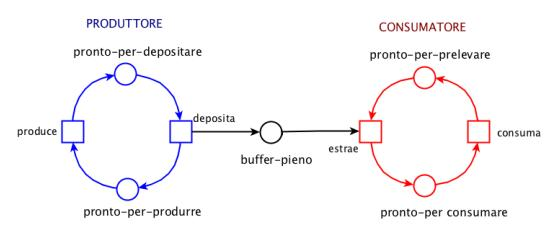
\includegraphics[scale = 0.7]{img/prod.jpg}
    \caption{Produttore e Consumatore}
  \end{figure}
  Lo stato globale del sistema è dato da una
  collezione di stati locali. Per segnare tali condizioni mettiamo un punto
  pieno dentro il cerchio e queste condizioni ``abilitano'' i vari eventi:
  \begin{figure}[h]
    \centering
    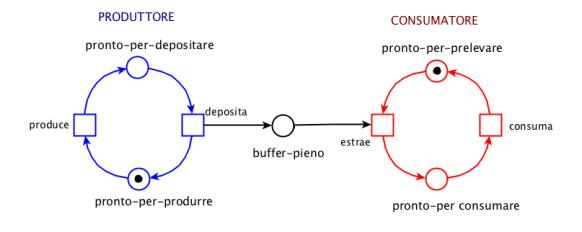
\includegraphics[scale = 0.7]{img/prod1.jpg}
    \caption{Uno stato globale Produttore e Consumatore dove l’evento\textit{
        produce} è l’unico abilitato} 
  \end{figure}
  Si può arrivare ad una \textit{configurazione} dove, per esempio, sia l'evento
  \textit{produce}, del produttore, che l'evento \textit{preleva}, del
  consumatore, sono abilitati. Si ha quindi che i due eventi possono occorrere
  in modo \textbf{concorrente} infatti i due eventi sono \textbf{indipendenti}
  in quanto condizionati da \textbf{precondizioni e postcondizioni completamente
    disgiunte}. Due eventi che occorrono in maniera concorrente lo possono fare in
  qualsiasi ordine, non si ha infatti una sequenza temporale specifica tra i
  due. \\
  In questo sistema quindi siano solo stati locali ed eventi localizzati e non
  stati ed eventi globali. Un evento dipende solo dalle sue precondizioni e
  dalle sue postcondizioni.\\
  \textit{Se rappresentiamo con delle marche le condizioni vere possiamo
    simulare il comportamento del sistema con il \textit{gioco delle marche} che
    mostra come l'evoluzione delle condizioni avviene all'occorrenza degli
    eventi.} \\
  La simula di un tale sistema può comunque avvenire con un sistema di
  transizioni etichettato, ovvero con un automa a stati finiti, che rappresenta
  gli stati globali corrispondenti alle diverse combinazioni di stati locali che
  di volta in volta sono veri. Gli archi vengono etichettati con gli eventi che
  comportano un cambiamento di stato globale:
  \begin{figure}[H]
    \centering
    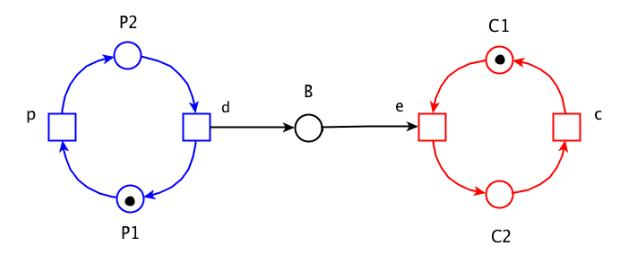
\includegraphics[scale = 0.7]{img/prod3.jpg}
    \caption{Semplificazione della nomenclatura del sistema per praticità}
    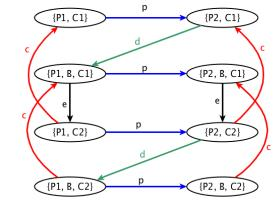
\includegraphics[scale = 0.8]{img/prod2.jpg}
    \caption{Rappresentazione del sistema con un automa a stati finiti che
      rappresenta stati globali}
  \end{figure}
\end{esempio}
Passiamo ora alla formalizzazione di questi aspetti.\\
\begin{definizione}
  Una \textbf{rete elementare} è definita come una tripla:
  \[N=(B,E,F)\]
  dove:
  \begin{itemize}
    \item $B$ è un insieme finito di \textbf{condizioni}, ovvero \textit{stati
      locali}, preposizioni booleane etc$\ldots$. Vengono rappresentate con un
    cerchio 
    \item $E$ è un insieme finito di \textbf{eventi}, ovvero trasformazioni
    locali di stato e \textit{transizioni locali}. Vengono rappresentate con un
    quadrato 
    \item $F$ è una \textbf{relazione di flusso} che connette condizioni ad
    eventi ed eventi a condizioni. Si ha quindi che:
    \[F\subseteq (B\times E)\cup(E\times B)\]
    Le relazioni di flusso sono rappresentate da archi orientati. Inoltre la
    relazione di flusso è tale per cui non esistano \textbf{elementi isolati},
    in quanto non avrebbero senso, in un tale sistema, eventi isolati (che non
    modificherebbero mai una condizione) o condizioni isolate (che non
    verrebbero mai modificate da un evento). Si ha, formalmente, che: 
    \[dom(F)\cup ran(F)=B\cup E\]
    \textbf{chiedere per formula sopra}
  \end{itemize}
  Si ha che:
  \[B\cap E = \emptyset\]
  \[B\cup E \neq \emptyset\]
  Ovvero gli insiemi delle condizioni e degli eventi sono tra loro disgiunti e
  non vuoti.\\
  Sia ora $x$ un elemento qualsiasi della rete, ovvero $x$ può essere o una
  condizione o un evento, formalmente:
  \[x\in B\cup E\]
  si ha che:
  \begin{itemize}
    \item $^\bullet x=\{y\in X:\,(y,x)\inF\}$ rappresenta l'insieme di tutti gli
    elementi $y$ che sono connessi dalla relazione di flusso ad $x$, ovvero si
    ha un arco da $y$ a $x$. Sono quindi i \textbf{pre-elementi} di $x$, ovvero
    le \textit{precondizioni}, se $x$ è un evento, o i \textit{pre-eventi}, se
    $x$ è una condizione
    \item $x^\bullet=\{y\in X:\,(x,y)\inF\}$ rappresenta l'insieme di tutti gli
    elementi $y$ che sono connessi dalla relazione di flusso a partire da $x$,
    ovvero si ha un arco da $x$ a $y$. Sono quindi i \textbf{post-elementi} di
    $x$, ovvero le \textit{postcondizioni}, se $x$ è un evento, o i
    \textit{post-eventi}, se $x$ è una condizione
  \end{itemize}
  Posso estendere questa notazione ad insiemi di elementi. Sia $A$ un insieme
  qualsiasi di elementi, che possono quindi essere sia condizioni che eventi:
  \[A\subseteq B\cup E\]
  Si ha quindi che i pre-elementi dell'insieme $A$ sono rappresentati con:
  \[^\bullet A=\cup_{x\in A} ^\bullet x\]
  ovvero l'unione dei pre-elementi di ogni singolo elemento dell'insieme $A$.\\
  Analogamente si ha che i post-elementi dell'insieme $A$ sono rappresentati
  con: 
  \[A^\bullet=\cup_{x\in A} x^\bullet\]
  ovvero l'unione dei post-elementi di ogni singolo elemento dell'insieme $A$.
  \textit{Nelle reti c'è sempre una relazione di \textbf{dualità} tra due elementi, per
    esempio tra condizioni ed eventi, tra pre-eventi e post-eventi, tra
    pre-condizioni e post-condizioni. Inoltre si ha la caratteristica della
    \textbf{località}, quindi si hanno stati locali e trasformazioni di stato
    locali}
\end{definizione}
La rete $N=(B,E,F)$ descrive la \textit{struttura statica del sistema}, il
comportamento é definito attraverso le nozioni di \textbf{caso (o
  configurazione)} e di \textbf{regola di scatto (o di transizione)}.\\
Una rete può anche essere suddivisa in sotto-reti, seguendo l'esempio sopra si
potrebbe avere una sotto-rete per il produttore, una per il consumatore e anche
una per il buffer.\\
\begin{definizione}
  Un \textbf{caso} (o \textbf{configurazione}) é un insieme di condizioni
  $c\subseteq B$ che rappresentano l’insieme di condizioni vere in una certa
  configurazione del sistema, un insieme di \textbf{stati locali} che
  collettivamente individuano lo \textbf{stato globale} del sistema.\\
  Graficamente le condizioni vere presentano un puntino in mezzo al cerchio
  mentre le condizioni false solo un cerchio vuoto
\end{definizione}
\begin{definizione}
  Sia $N=(B,E,F)$ una rete elementare e sia $c\subseteq B$ una certa
  configurazione (non serve quindi necessariamente conoscere tutto lo stato del
  sistema). La \textbf{regola di scatto} mi permette di stabilire quando
  un evento $e\in E$ è abilitato, ovvero può occorrere, in $c$ sse:
  \[^\bullet e\subseteq c \mbox{ e } e^\bullet \cap c = \emptyset\]
  ovvero sse tutte le precondizioni dell'evento sono vere (e quindi sono
  contenute nella configurazione $c$) e sse tutte le postcondizioni sono false
  (quindi non si hanno intersezioni tra le postcondizioni e la
  configurazione). \\
  L'occorrenza (l'abilitazione) di $e$ in $c$ si denota con la scrittura:
  \[c[e >\]
  Se un evento $e$ è abilitato in $c$, ovvero $c[e >$, si ha che quando $e$
  occorre in $c$ genera un nuovo caso $c'$ e si usa la notazione:
  \[c[e > c'\]
  Si ha quindi che $c'$ è così calcolabile:
  \[c'=(c-^\bullet e)\cup e^\bullet\]
  Ovvero togliendo da $c$ tutte le precondizioni dell'evento $e$ e aggiungendo
  quindi tutte le postcondizioni di $e$
\end{definizione}
Le reti si basano sul \textbf{principio di estensionalità}, ovvero sul fatto che
il cambiamento di stato è locale:
\begin{center}
  \textit{un evento è completamente caratterizzato dai cambiamenti che produce
    negli stati locali, tali cambiamenti sono indipendenti dalla particolare
    configurazione in cui l’evento occorre.}
\end{center}
L'importante è che le precondizioni di un evento siano vere e le postcondizioni
false (siamo comunque interessati solo alla validità delle condizioni che
riguardano l'evento).
\newpage
\begin{esempio}
  Vediamo un esempio esplicativo dove l’evento $e$ è l'unico abilitato, ovvero
  le sue precondizioni sono vere e le sue postcondizioni sono false.\\
  Lo scatto di $e$ rende le precondizioni false e le postcondizioni vere,
  mentre le altre condizioni rimangono inalterate:
  \begin{figure}[H]
    \centering
    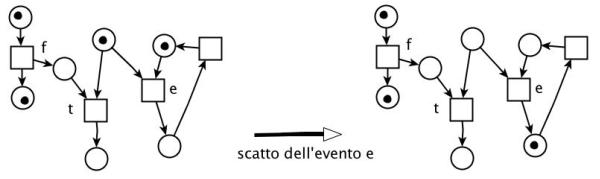
\includegraphics[scale = 0.6]{img/est.jpg}
  \end{figure}
  Si nota quindi che lo scatto dell'evento $e$ riguarda solo le precondizioni e
  le postcondizioni di quel dato evento, come ci ricorda il principio di
  estensionalità 
\end{esempio}
\begin{definizione}
  Sia $N=(B,E,F)$ una rete elementare. Possiamo definire due tipologie di rete:
  \begin{enumerate}
    \item $N$ è definita \textbf{semplice} sse:
    \[\forall x,y \in B\cup E,\,\, (^\bullet x = ^\bullet y)\wedge (x^\bullet =
      y^\bullet)\Rightarrow x = y\]
    Ovvero per ogni coppia di elementi (che siano quindi eventi o condizioni) se
    i loro pre-elementi e i loro post-elementi coincidono allora non ha senso
    distinguere $x$ e $y$.
    \begin{figure}[H]
      \centering
      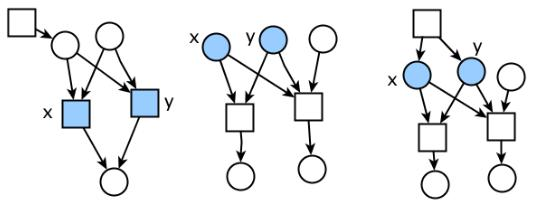
\includegraphics[scale = 0.5]{img/sem.jpg}
      \caption{Esempi di reti \textbf{non} semplici}
    \end{figure}
    \newpage
    \item $N$ è definita \textbf{pura} sse:
    \[\forall e \in E:\,\,^\bullet e \cap e^\bullet = \emptyset\]
    Ovvero se per ogni evento non esiste una precondizione che sia anche
    postcondizioni. Si ha quindi un \textbf{cappio} (detto anche \textbf{side
      condition}) tra un evento e una condizione. Avere questa situazione
    comporta che l'evento non può scattare in quanto la condizione che per lui è
    sia una precondizione che una postcondizioni non può essere
    contemporaneamente vera e falsa, l'evento non potrà mai scattare e quindi
    non potrà mai essere osservato. Non avrebbe quindi senso modellarlo
    \begin{figure}[H]
      \centering
      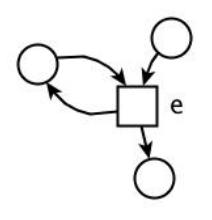
\includegraphics[scale = 0.5]{img/pura.jpg}
      \caption{Esempio di rete \textbf{non} pura}
    \end{figure}
  \end{enumerate}
\end{definizione}
\begin{definizione}
  Data una rete elementare $N=(B,E,F)$ e sia $U \subseteq E$ un sottoinsieme di
  eventi e siano $c,c_1,c_2\in B$ tre configurazioni. Si ha che:
  \begin{itemize}
    \item $U$ è un \textbf{insieme di eventi indipendenti} sse:
    \[\forall e_1,e_2\in U:\,\,e_1\neq e_2\Rightarrow (^\bullet e_1\cup
      e_1^\bullet)\cap  (^\bullet e_2\cup e_2^\bullet) = \emptyset\]
    ovvero per ogni coppia distinta di eventi nell'insieme $U$ si ha che le
    precondizioni e le postcondizioni dei due eventi sono completamente
    disgiunte.
    \item $U$ è un \textbf{passo abilitato}, ovvero un insieme di \textit{eventi
      concorrenti} in una certa configurazione $c$, che si indica con:
    \[c[U>\]
    sse:
    \[U \mbox{ è un insieme di eventi indipendenti } \wedge\,\, \forall e\in
      U:\,\, c[e>\]
    $U$ quindi deve essere un insieme di eventi indipendenti e ogni evento in
    $U$ è abilitato in $c$, quindi le sue precondizioni sono vere e le sue
    postcondizioni sono false. Si ha quindi che $U$ è un insieme di eventi
    abitati in maniera concorrente in $c$
    \item $U$ è un \textbf{passo} dalla configurazione $c_1$ alla configurazione
    $c_2$, che si indica con:
    \[c_1[U > c_2\]
    sse:
    \[(c_1[U) \wedge \Big(c_2=(c_1-^\bullet U)\cup U^\bullet\Big)\]
    ovvero sse $U$ è un passo abilitato in $c_1$ e lo scatto degli eventi in $U$
    porta alla configurazione $c_2$ che si ottiene togliendo da $c_1$ l'insieme
    delle precondizioni degli eventi in $U$ e aggiungendo quindi l'insieme delle
    postcondizioni degli eventi in $U$
  \end{itemize}
\end{definizione}
\begin{esempio}
  Riprendiamo l'esempio del produttore e del consumatore.\\
  Sia dato il sistema $\Sigma$ che modella produttore e consumatore
  \begin{figure}[H]
    \centering
    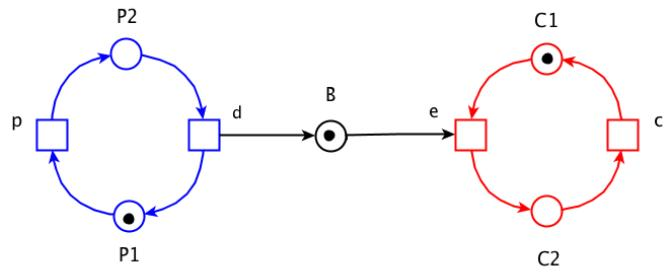
\includegraphics[scale = 0.6]{img/prod5.jpg}
  \end{figure}
  Si hanno:
  \begin{itemize}
    \item $\{p,e\},\{p,c\},\{d,c\}$ esempi di insiemi di eventi indipendenti
    \item $\{p,e\}$ che è un passo abilitato in $\{P_1,B,C_1\}$
    \item $\{P_1,B,C_1\}[\{p,w\}>\{P_2,C_2\}$ ovvero lo scatto del passo
    $\{p,e\}$ ci porta in $\{P_2,C_2\}$
  \end{itemize}
\end{esempio}
Diamo ora una definizione formale di \textbf{sistema elementare}.
\begin{definizione}
  Un \textbf{sistema elementare} $\Sigma=(B,E,F;c_{in})$ è definito come una
  rete $N=(B,E,F)$ e a cui è associato un caso iniziale, una configurazione
  iniziale, ovvero un sottoinsieme di condizioni che rappresentano lo stato
  iniziale da cui inizia la computazione e l'evoluzione del sistema. Formalmente
  il caso iniziale si indica con $C_{in}\in B$ 
\end{definizione}
\begin{definizione}
  Dato un sistema elementare $\Sigma=(B,E,F;c_{in})$ si indica con $C_\Sigma$
  l'insieme dei \textbf{casi raggiungibili} da tale sistema a partire dal caso
  iniziale $c_{in}$.\\
  Formalmente l'insieme dei casi raggiungibili è il di piccolo sottoinsieme
  dell'insieme delle parti di $B$, ovvero $2^B$, tale che:
  \begin{itemize}
    \item $c_{in}\in C_\Sigma$, ovvero sicuramente il caso iniziale appartiene
    all'insieme dei casi raggiungibili
    \item se $c\in C_\Sigma,\,U\subseteq E$ e $c'\subseteq B$ sono tali che
    $c[U>c'$ allora $c'\in C_\Sigma$, ovvero se ho un generico caso $c$ che
    appartiene ai casi raggiungibili, se ho un insieme di eventi $U$ tale che
    questo insieme di eventi (che abbiamo visto essere indipendenti, per la
    definizione di passo abilitato) è abilitato
    in $c$ in un unico passo e la sua occorrenza mi porta in $c'$, allora anche
    $c'$ appartiene a $C_\Sigma$. 
  \end{itemize}
  Questa è una definizione data per \textbf{induzione strutturale}, nel primo
  punto si ha la base, nel secondo l'ipotesi e la conseguenza
\end{definizione}
\begin{definizione}
  Dato un sistema elementare $\Sigma=(B,E,F;c_{in})$ si indica con $U_\Sigma$
  l'\textbf{insieme dei passi} di $\Sigma$, ovvero di tutti i possibili insiemi
  di eventi indipendenti che possono occorrere in qualche caso. Formalmente:
  \[U_\Sigma =\{U\subseteq E\,|\,\exists\, c,c'\in C_\Sigma :\, c[U>c'\}\]
  Ovvero l'insieme dei sottoinsiemi di eventi tali per cui esistano due casi
  raggiungibili in $C_\Sigma$ e $U$ è abilitato in $c$ e il suo scatto mi porta
  in $c'$.
\end{definizione}
% 4.27
\end{document}


% LocalWords:  postcondizioni LocalWords estensionalità jpg img sse pre sem
% LocalWords:  side condition prod
